\section{Motor Control Unit}

The MCU's task is to control the motor as efficiently as possible. In order to do so monitoring both the speed and power usage is necessary to regulate the current efficiently to the motor.

In extenstion it's also the MCU's task to log information about the BMS output, it's own measurements and all inputs from the driver, thereby making it possible to debug and analyze the run. 

\subsection{Design}

First step is to find out what solution that should be used, to build the MCU. 

\begin{enumerate} %\fxnote{Det første var vel og finde ud af hvad der var krævet at MCU'ens software (Forskellige kører algoritmer, EEPROM osf.) - JH}
	\item \textbf{Get the best efficiency}\\
	To get the best efficiency a LUT must be implemented so the MCU can look up power usage for a specific speed. To make it even more efficiency a burn and coast algorithm must also be implemented. \\
	\item \textbf{Get information from other devices (only BMS for now) in the AU2}\\
	To get information from the BMS a communication has to been made. To do this a CAN connection are made to the BMS. The reason what a CAN are choose is because it work as bus connection and more devices can be linked together in the future version.\\
	\item \textbf{Log information and events}\\
	A logger has to be design, so what information from a run can be analyze. Also log events so it is easier to find bugs.\\
	\item \textbf{Can be control by the driver}\\
	It is important what it is possible to start or stop the motor. To do this a button is implemented so it is possible to tell MCU if the car should drive or not. Therefor this also has to be designed.\\
	\item \textbf{Save local sitting}\\
	The MCU must save local sittings in case that the a short power failure or the car are shutdown. Example PID parameter.\\
\end{enumerate}

Next step is to design a class diagram to get a better overview of have the classes should be linked. See figure \vref{fig:Class_diagram_MCU}.

\begin{figure}[H]
	\centering
	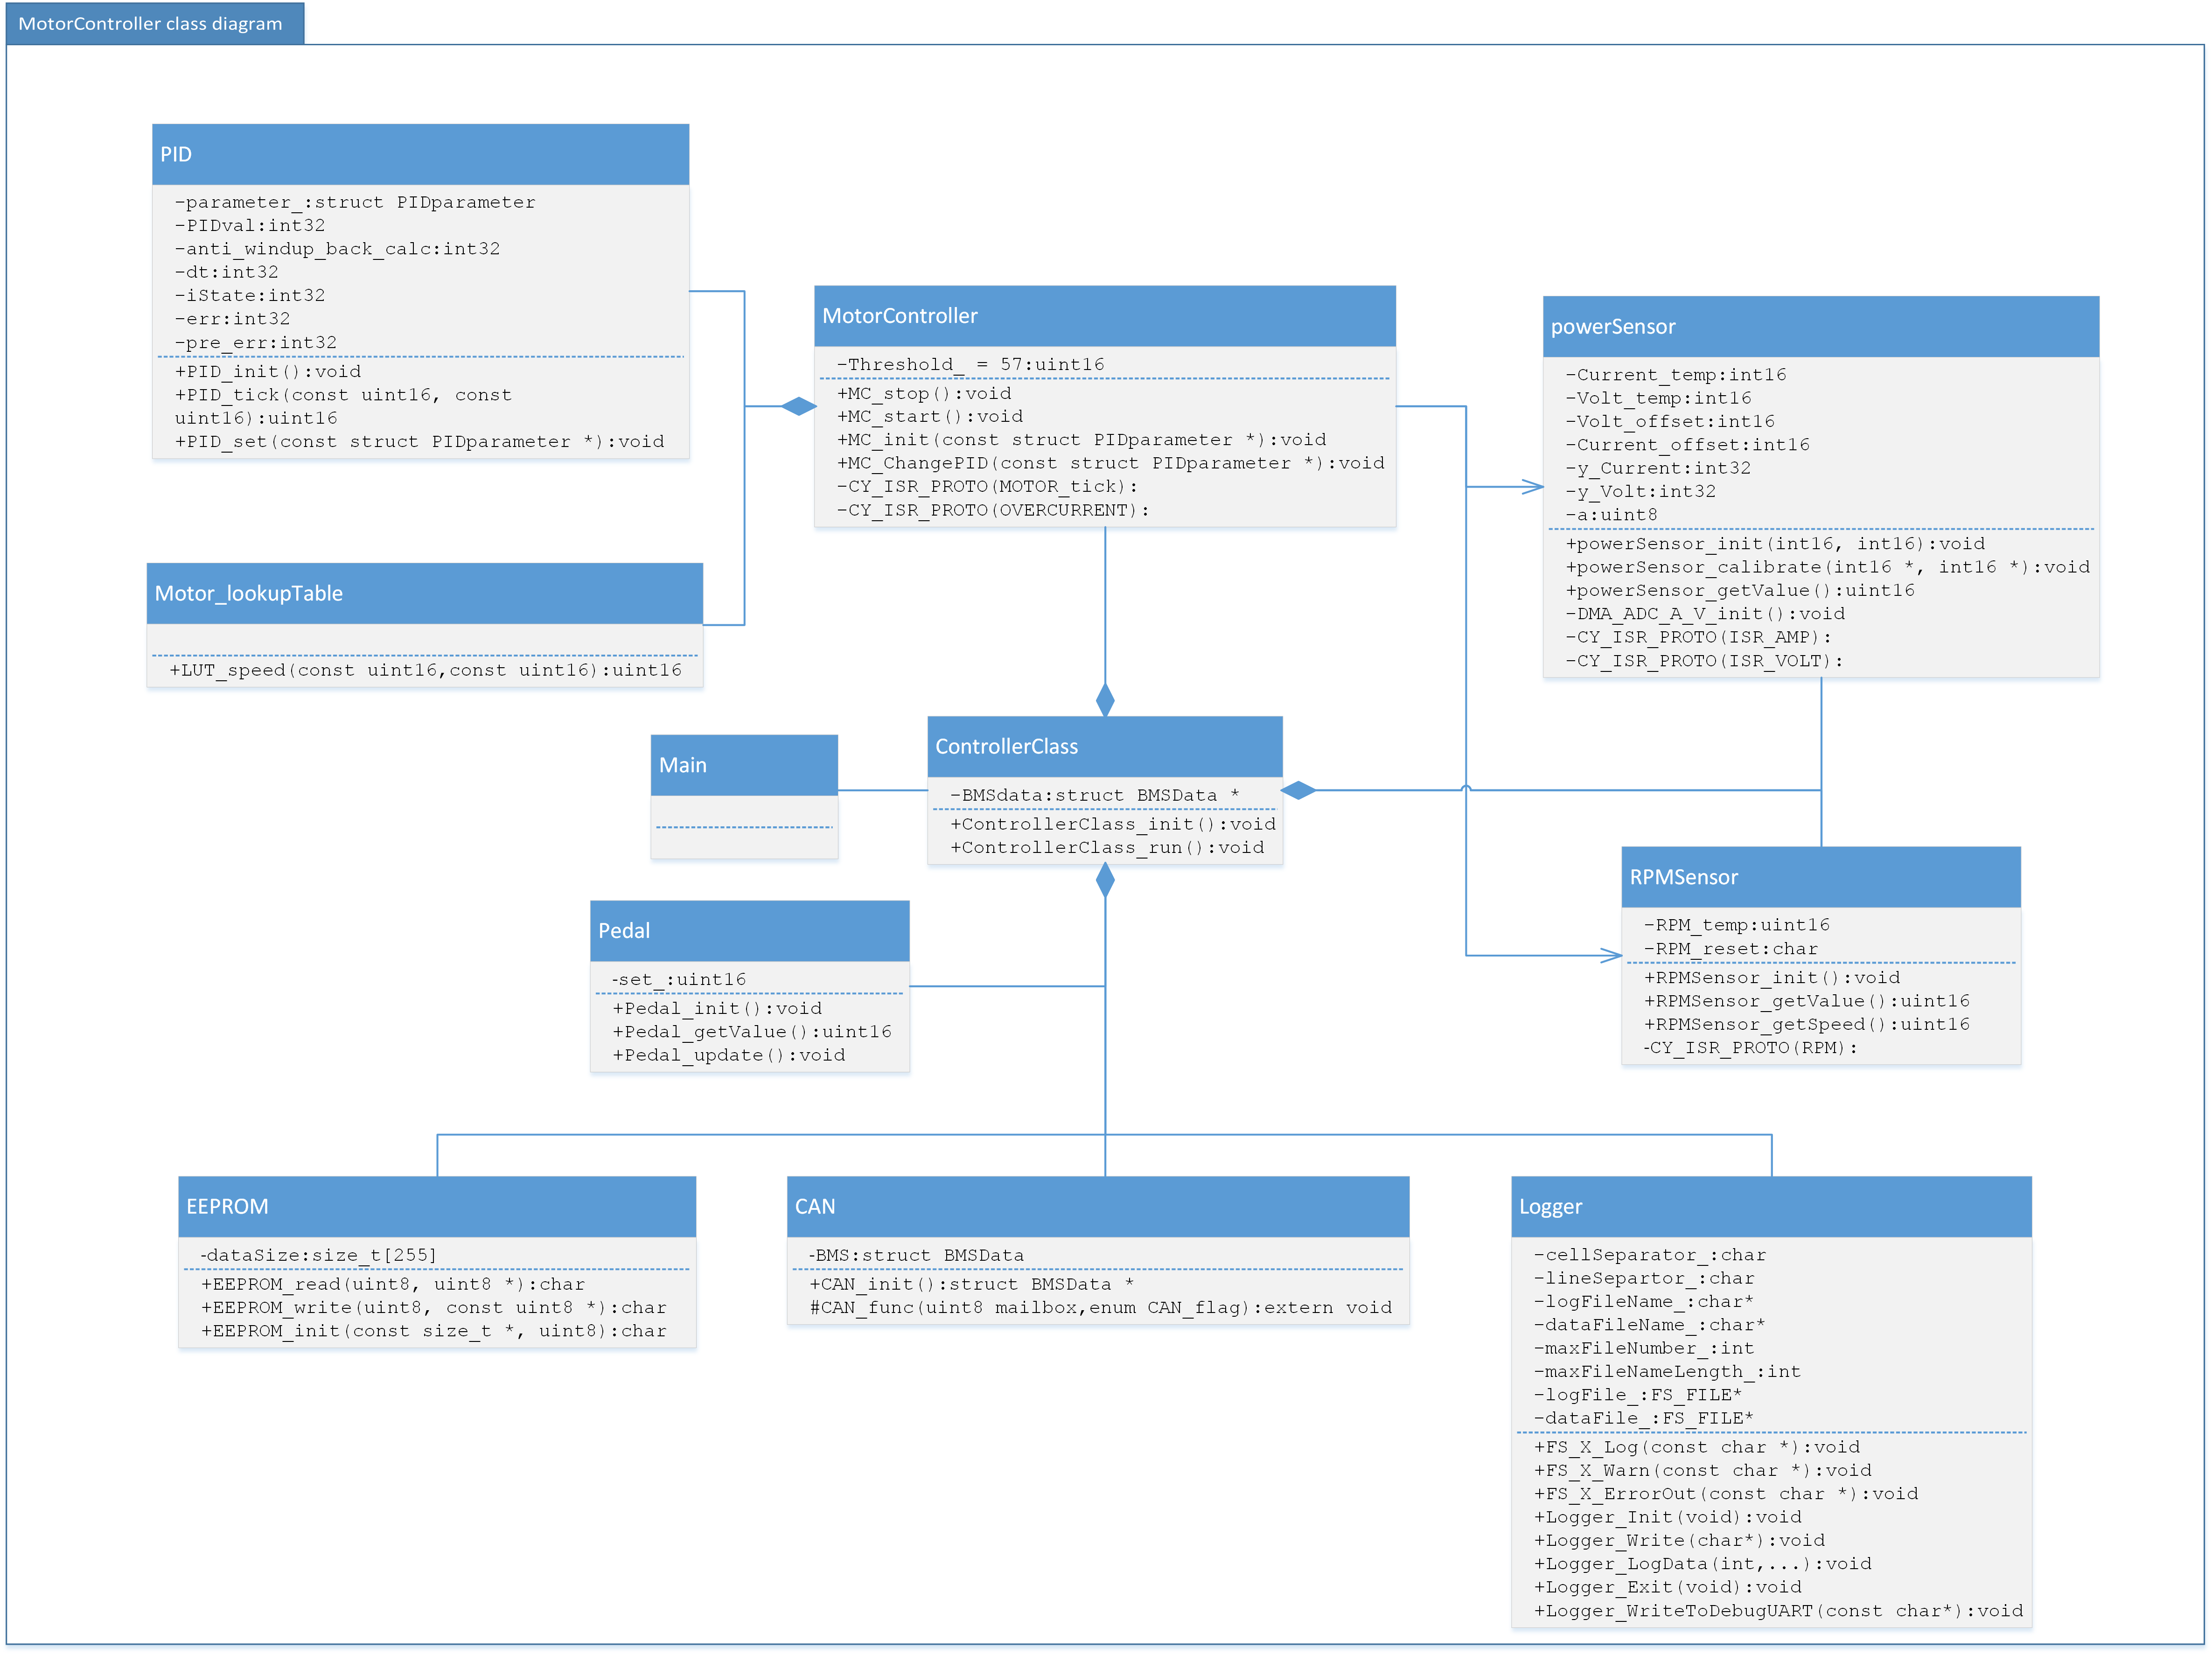
\includegraphics [width=6in]{../Documentation_AU2/Software/Pictures/class-diagram.png}
	\caption{Class diagram of the MCU}
	\label{fig:Class_diagram_MCU}
\end{figure}

\subsection{Implementation}

In the implementation process a lot of decision have to be made. The biggest question is there should the different things be implemented. software level, top-design level or circuit design level. \\

\begin{enumerate} %\fxnote{Det første var vel og finde ud af hvad der var krævet at MCU'ens software (Forskellige kører algoritmer, EEPROM osf.) - JH}
	\item \textbf{Look Up Table}\\
	The implementation process of the LUT. Some decision should be made before implementation.\\
	\subitem \textit{What kind of LUT?}\\
	A 2D-LUT are implemented so the MCU has two Look Up tables, one then it is accelerating and one to then it has to hold a constant speed.\\
	\subitem \textit{How to generate the LUT}\\
	To generate the LUT (see figure \vref{fig:LUT_plot}) a Matlab script\cite{LUTscript} is made. Where it is just to read from a efficiency diagram for the AU transmission from motor to road  (see \cite{BAC_zenith33}) and insert the best ramp for the acceleration and constant. There the script will create a header file with a 2D LUT.\\
	This will also make it very easy to load a new LUT into the MCU. Just have recompile the MCU.\\
	\subitem \textit{Implementation to the PSoC}\\
	To use the header file a function is made to read from the LUT. It is the function job to also find out what table it should use.\\	
	\item \textbf{burn and coast}
	This is implemented in the motorController class as a state-machine. There it switch between using the accelerating LUT and then hit the wanted speed it turn off the motor to it has fall below a specify speed value where it is switching back again. 
	\item \textbf{Get information from other devices (only BMS for now) in the AU2}\\
	To implement this. The build in CAN in the PSoC 5LP is used. 
	\item \textbf{Log information and events}\\
	To log a SD card is implemented so to read and write from it a library was used. The library "emFile" made it possible to read or write from and to a fat32 devices.\\
	\item \textbf{Can be control by the driver}\\
	This was implemented just with a simple button, so the software implementation is just to read from a status register to see if it pressed or not.\\
	\item \textbf{Save local sitting}\\
	The build in EEPROM on the PSoC 5LP is used a local ROM. There the PSoC creator provided a lot of help function to access the EEPROM. Still a class is made to handle where the saved data is placed or where to read from the EEPROM. It can also control what it is not reading some random information.\\ 
	\item \textbf{The regulator}\\
	\subitem \textit{What kind of regulator?}\\
	A PID regulator because it has to be easy for everyone to tune. And it is also easy to calculate some PID constants, but because AU2 is not complete and has not got enough data of the car this isn't possible yet.\\
	\subitem \textit{Where to implement the PID regulator}\\
	The reason that it is not implemented in the digital filter block what would be the most optimal solution. Is because then implemented it on the software level it is easy to change the PID constant without recompiling. Of course then it has been tested and the PID constants are found, it would be smarter and less power consuming to use the digital filter block.\\
	\subitem \textit{What to regulate}
	The input comes from the LUT. The feedback are the product from voltage- and current-sensor. The regulator will then regulate the motor with a PWM signal.\\
	To get data from the sensor a DMA is setup. So no need for a interrupt routine every time a conversion is done. This will also save a lot of CPU time\\
\end{enumerate}

\begin{figure}[H]
	\centering
	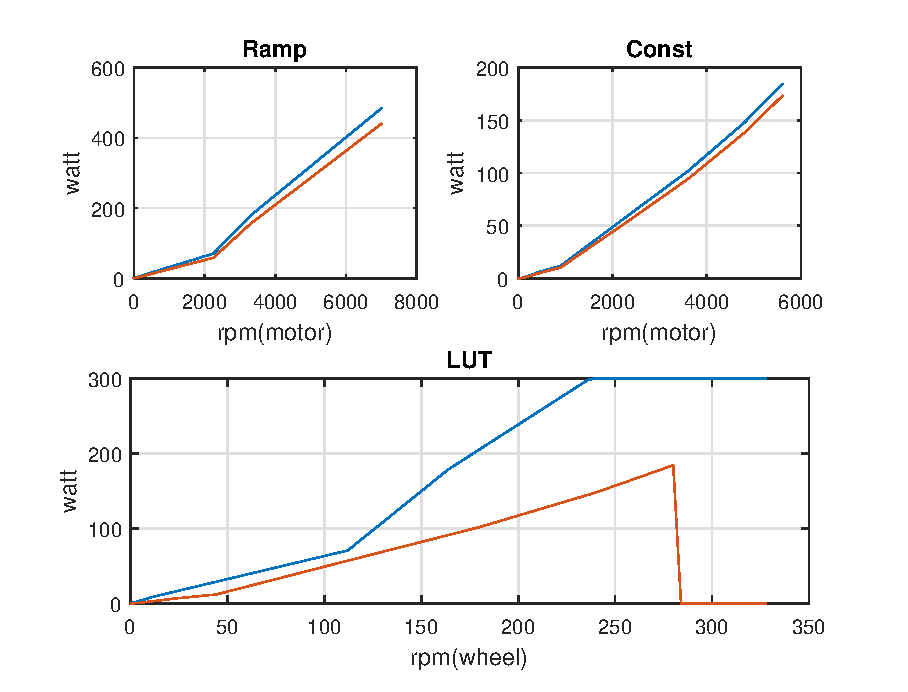
\includegraphics [width=6in]{../Documentation_AU2/Software/Pictures/LUT.eps}
	\caption{LUT plot - "Ramp" is the power use for a specific speed(red = without power loose, blue = with power loose) this table are used then accelerating. "Const" is the same but just then the car should hold a constant speed(red = without power loose, blue = with power loose). "LUT" is the 2D-look Up Table(blue = accelerating; red constant speed)}
	\label{fig:LUT_plot}
\end{figure}


\subsection{Test}

The Motor Control unit has yet been tested because of some problem with the PCB. But all sensor and regulator has been tested with a simple setup figure \vref{fig:PSOC_test} only using a PSoC and a Analog discovery. So it should be ready for AU2 then it is finish.

\begin{figure}[H]
	\centering
	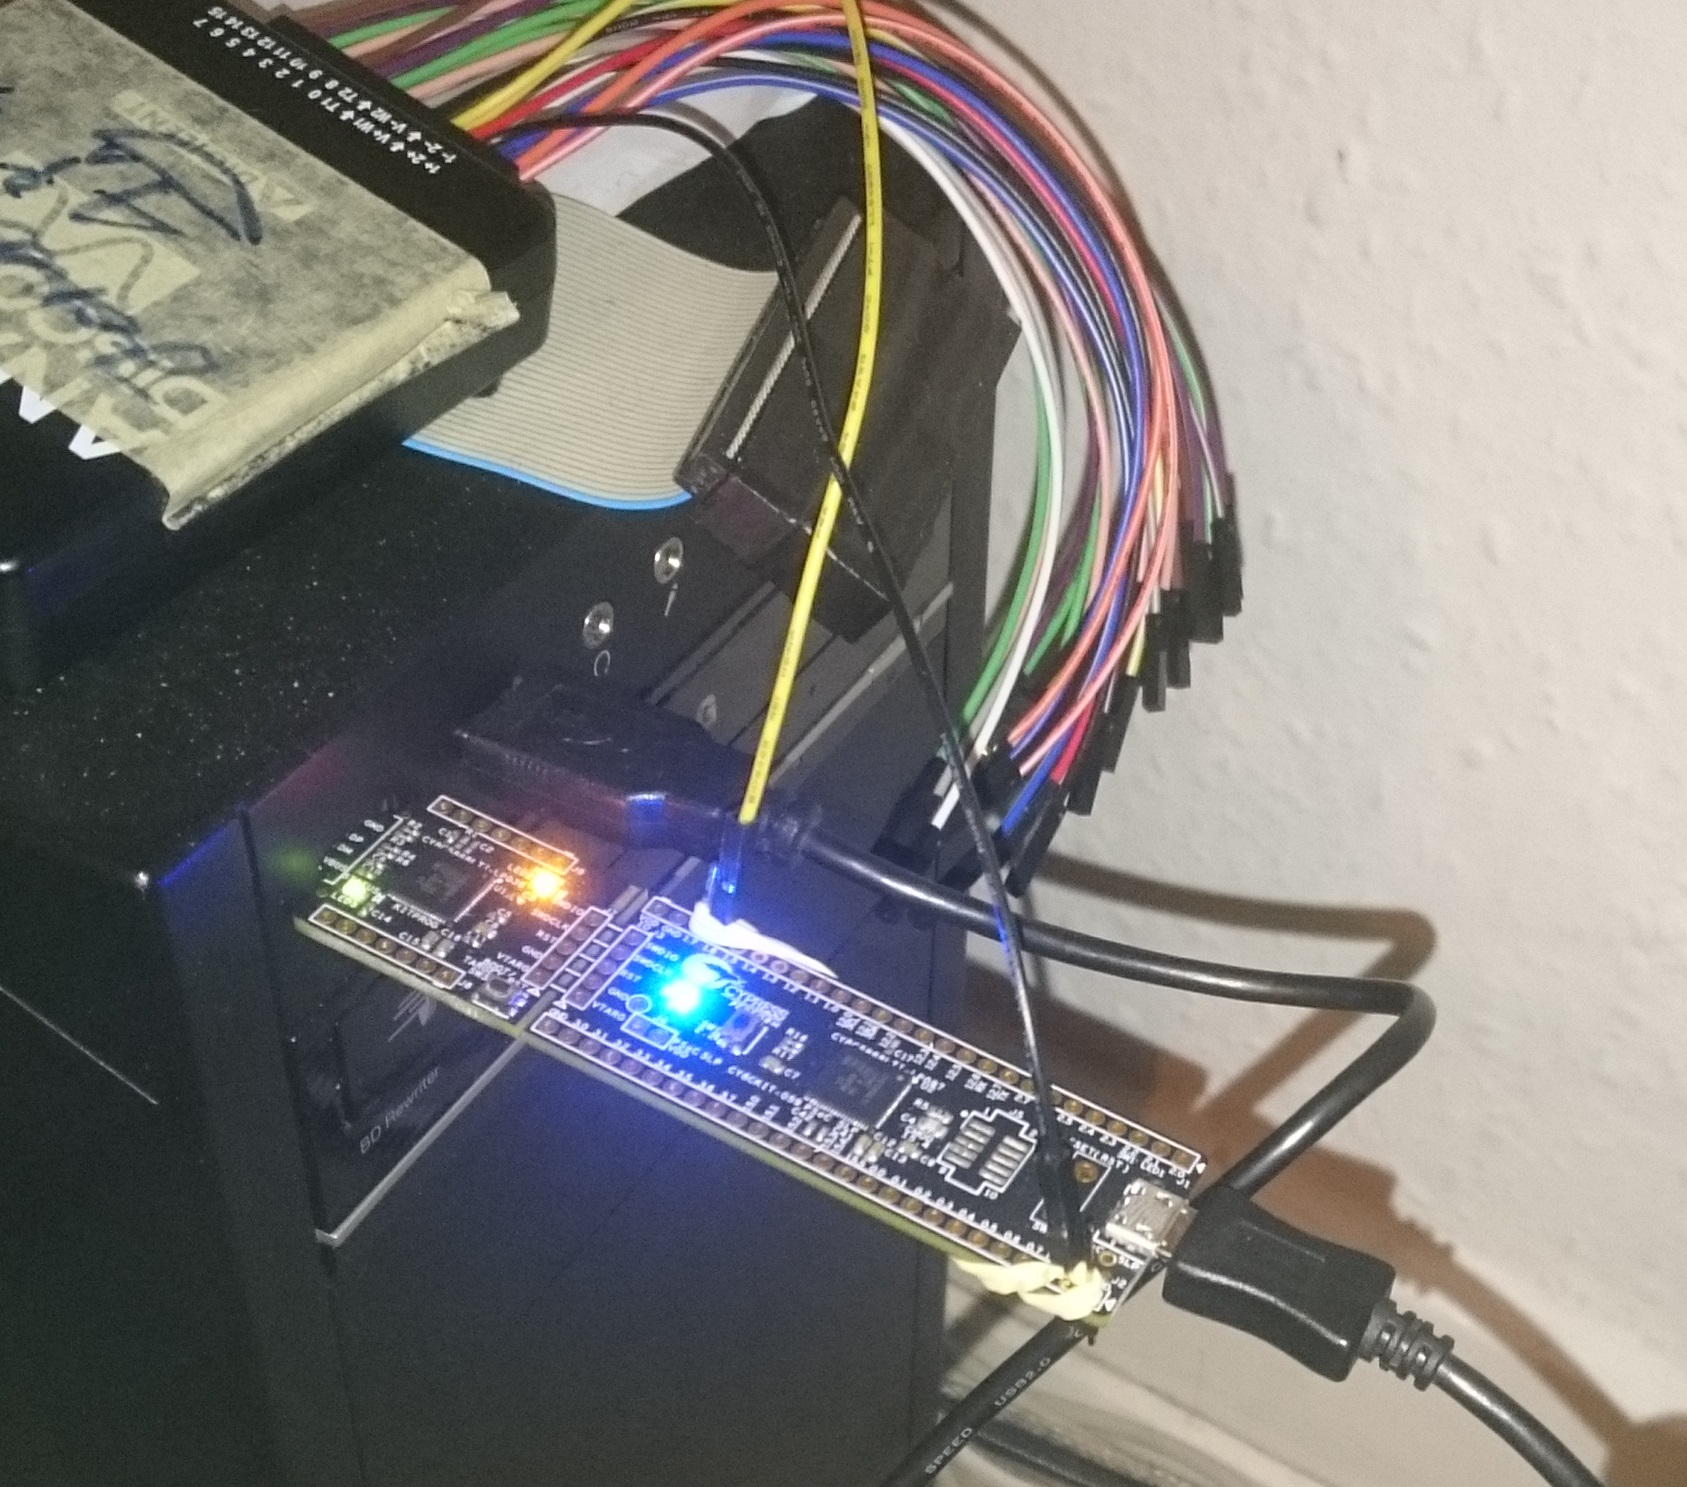
\includegraphics [width=4in]{SubPages\Images\SoftwareTestPSoC.jpg}
	\caption{A simple test setup for the PSoC. Note more test has been made, this is just a picture of one of the first test that has been made.}
	\label{fig:PSOC_test}
\end{figure}

